\documentclass[9pt,24pt,twocolumn]{article}
\usepackage[utf8]{inputenc}
\usepackage[spanish]{babel}
\usepackage{amsmath}
\usepackage{amsfonts}
\usepackage{amssymb}
\usepackage{graphicx}
\usepackage[left=1.5cm,right=1.5cm,top=1.5cm,bottom=2.4cm]{geometry}
\author{Correa Barcos Valentina, Pajaro Daniel, Restrepo Aguilera Yulissa
\\
\\
\textit{Facultad de Ingeniería, Universidad Tecnológica de Bolívar}
\\
{\textit{Cartagena, Bolívar}}
\\
\\{\small {valencorreabarco@hotmail.com}}
\\{\small {yulissatatiana@gmail.com}}
}

\date {}
{\title{{\Huge ENCRIPTACIÓN Y DESENCRIPTACIÓN DE DATOS}}}

\begin{document}

\maketitle

\emph{Resumen— El cifrado es el proceso de ocultar datos o archivos mediante el uso de una clave o contraseña que consigue que, quienes accedan a ellos sin la contraseña adecuada, no puedan encontrar ninguna utilidad en los mismos, puesto que resulta difícil descifrar su contenido. De igual manera estos procesos se pueden realizar de dos maneras (simétricas o clave privada y asimétricas o clave pública), todos con el fin de buscar una mejor seguridad de nuestros datos.}
\\

\begin{center}
{I. INTRODUCCIÓN}
\end{center}

{Es necesario, crear diferentes mecanismos, dirigidos a garantizar la confidencialidad y autenticidad de los documentos electrónicos, todo ello es parte de una nueva tecnología denominada Criptografía. Se aborda el tema de la seguridad informática y las diversas variantes criptográficas: simétrica y asimétrica.}
\\

{Los datos críticos pueden ser solo un pequeño porcentaje de toda la información que la empresa almacena, pero es la más valiosa. Y todo elementos o datos prioritarios se deben vigilar y rastrear para el bien de la empresa o compañía.}
\\

{Este artículo consiste en la investigación de la existencia de la desprotección de los datos críticos y/o confidenciales en una empresa, dándole su debida solución con un programa de encriptación de información y archivos.}
\\

\begin{center}
{II. CRIPTOGRAFIA}
\end{center}

{El uso de la encriptación o también llamado criptografía se usa desde la Antigua Grecia. Es del griego de donde viene el nombre de la ciencia del cifrado, la criptografía: krypto “ocultar” y graphos “escribir”, es decir escritura oculta.}
\\

{La encriptación es un conjunto de técnicas que tratan sobre la protección de la información frente a observadores no autorizados, ocultando datos o archivos mediante el uso de una clave. Ha sido usada a través de los años para mandar mensajes confidenciales con el propósito que sólo las personas autorizadas puedan entenderlos. A este proceso de “esconder” y poder recibir el archivo “escondido” se llama encriptación y desencriptación respectivamente.}
\\

{Pero la confidencialidad no es lo único que permite la criptografía. También resuelve otros problemas de seguridad, como certificar la "autenticidad" (firma de mensajes) e "integridad" (chequear que la información transmitida no ha sido modificada) de la información.}
\\

{Actualmente la criptografía ha evolucionado hacia sistemas mucho más complicados de romper y se usa a diario para aplicaciones diversas como conexiones seguras a ciertas páginas de Internet a las que se envía información sensible, almacenamiento de datos seguro, o firma electrónica. Existen dos tipos fundamentales de criptosistemas:}
\\

\textit{A.  Criptosistemas simétricos o de clave privada:}

{En este tipo de criptografía se utiliza la misma clave para cifrar y para descifrar (clave secreta), que debe ser solamente conocida por las partes autorizadas para este proceso.}
\\

\begin{figure}[h]
  \centering
    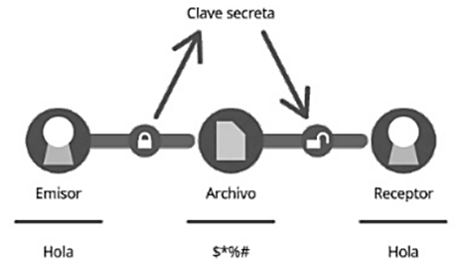
\includegraphics{simetrico1}
  \caption{Criptografía Simétrica(Moraga, 2015)}
  \label{fig:sim}
\end{figure}


{La criptografía simétrica es considerada la más fácil, sin embargo, aunque los algoritmos son más sencillos y generalmente rápidos, tiene algunos problemas, como por ejemplo que necesitamos un "canal seguro" para transmitir o acordar la clave.}
\\

{Entre sus características encontramos las siguientes:}
\\

{• A partir del mensaje cifrado no se puede obtener el mensaje original ni la clave que se ha utilizado.}
\\

{• Se utiliza la misma clave para cifrar y descifrar el mensaje original, la clave no cambiara ni para el emisor ni para el receptor del mensaje.}
\\

{• Emisor y receptor deben haber acordado una clave común por medio de un canal de comunicación confidencial y es ahí donde radica el principal problema con los sistemas de cifrado simétrico no está ligado a su seguridad, sino al intercambio y distribución de claves.}
\\

\textit{B.  Criptosistemas asimétricos o de clave pública:}

{En cambio, este tipo de criptografía emplea una doble clave de forma que una cifra (clave pública) y la otra descifra (clave privada), y en muchos casos son intercambiables.}

\begin{figure}[h]
  \centering
    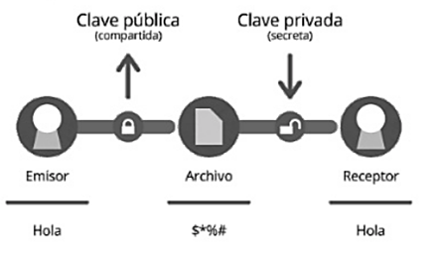
\includegraphics{asimetrico1}
  \caption{Criptografía Asimétrica(Moraga, 2015)}
  \label{fig:asim}
\end{figure}

{La criptografía asimétrica es más potente, y nos permite un servicio de autenticidad y asegurar la integridad de los mensajes, sin necesidad de transmitir una clave secreta o privada (solo es conocida o compartida la clave pública, que puede transmitirse por un canal inseguro pues no hay problema en que sea conocida).}
\\

{Algunas de sus características son las siguientes:}
\\

{• Se utilizan una pareja de claves denominadas clave pública y clave privada, pero a partir de la clave pública no es posible descubrir la clave privada.}
\\

{• A partir del mensaje cifrado no se puede obtener el mensaje original, aunque se conozcan todos los detalles del algoritmo criptográfico utilizado y aunque se conozca la clave pública utilizada para cifrarlo.}
\\

{• Emisor y receptor no requieren establecer ningún acuerdo sobre la clave a utilizar. El emisor se limita a obtener una copia de la clave pública del receptor, lo cual se puede realizar, en principio, por cualquier medio de comunicación, aunque sea inseguro.}
\\

{Como finalidad de la criptografía es poder garantizar el secreto entre la comunicación de dos remitentes, ya sea, personas u organizaciones, y además asegurar que la información que se envía sea real y confiable de dos maneras, que el remitente sea realmente quien dice ser y que el contenido del mensaje enviado, llamado criptograma, no haya sido modificado en su tránsito.}
\\

{En esta rama de la seguridad informática podemos definir el uso en su historia, siendo la criptografía muy antigua como lo es la escritura, pero ha tomado más fuerza hoy en día con sus aplicaciones en sistemas informáticos y los nuevos algoritmos de cifrado de la información asegurando así los pilares fundamentales sobre los que se basa la criptografía:}
\\

{-	Seguridad: asegurarse que el texto del mensaje solo pueda ser leído por el destinatario.}
\\

{-	Integridad: certeza que el mensaje no ha sufrido ninguna manipulación posterior de los datos.}
\\

{-	Autenticidad: certeza del remitente, acredita quien es su autor.}
\\

{Las claves usadas para el cifrado son combinaciones de símbolos, que pueden ser letras, números, signos de puntuación, etc. Por lo tanto, la seguridad está expuesta a posibles ataques en el momento de compartir los datos. Para evitar esto se debe tener en cuenta las siguientes reglas:}
\\

{a) Claves con gran longitud, necesitando mas recursos para cubrir todo el rango rápidamente y llegar a la clave.}
\\

{b)  Cambio regular de nuestra clave.}
\\

{c) Utilizar varios tipos de caracteres, para que sea aún mucho más difícil de adivinar.}
\\

{d)  No utilizar palabras de diccionario o nombres propios.}
\\

{Finalmente, entre las limitaciones de la criptografía está el hecho que este método tiende a degradarse con el tiempo, en donde los algoritmos se hacen más fáciles de quebrar debido al avance de la velocidad y potencia de los equipos de computación. Estos algoritmos criptográficos son vulnerables a los ataques de fuerza bruta (forzar a encontrar la clave de cifrado), la cual es más fácil de aplicar a medida que avanza el tiempo.}
\\

\begin{center}
{III. RIESGOS EN LA RED}
\end{center}

{El Internet ofrece infraestructura económica y cultural para facilitar muchas actividades humanas, aun así, las personas entran a varios sitios en los que agregan información personal que conlleva riesgos especialmente a niños por su inocencia en todo lo que encuentra en la red, así como los adolescentes. Todas las funcionalidades del Internet pueden contener algún riesgo:}
\\


\textit{A.  Riesgos relacionados con información:}

{La mayoría de las veces, las personas que utilizan Internet son poco protectoras de la información que comparten en la red. Dichos datos llegan a terceras personas con fines maliciosos como difundir, plagiar, difamar y amenazar.}
\\

\textit{B.  Riesgos relacionados con actividades económicas. }

{En la red se realizan una gran cantidad de actividades, por lo que, algunas de dichas actividades son relacionados con repercusión económica.}
\\

\textit{C.  Estándar:  }

{Las acciones o transacciones económicas pueden terminar en engaños y estafas al creer varios sitios web que llaman tu atención y así, puedas caer en su red de mentiras.}
\\

\textit{D.  Robos: }

{Al tener información especifica en sitios web puedes pasar por robo de identidad por programas malicioso que si lo tomamos desde una perspectiva de una empresa es una pérdida de dinero debido a la poca fiabilidad de la protección de datos en un sistema poco seguro que no cumple su objetivo.}
\\

\begin{center}
{IV.  PROBLEMÁTICA}
\end{center}

{El avance tecnológico de hoy en día nos facilita tanto las comunicaciones entre nosotros como la manipulación e intercambio de información para compartir información en recursos tecnológicos, centralizar determinados procesos y abaratar costes en prestación de servicios por las empresas. Estos avances permiten que los datos personales circulen de manera rápida y sean almacenados indefinidamente en algún lugar.}
\\

{El flujo de datos personales no solo influye auxiliar respecto de empresas, entidades o personas que utilizan o realizan diversas actividades con la información como por ejemplo apartar un tiquete de avión o comprar en Internet, pero estas no se han realizado sin costes de poner en peligro la vida privada de las personas.}
\\

{Para nadie es secreto que, sin demasiadas técnicas, la información puede ser objeto de un tratamiento ilícito, por lo que, sería una transferencia de datos sin consentimiento del propietario de dicha información violando sus derechos fundamentales constitucionalmente protegidos. De ahí la aparición de diversos modos de que estos ciber-ataques en la información sean dados.}
\\

{Con estos posibles ataques de robo de información que existen tanto en la red como fuera de ella, se hace de manera necesaria que cada empresa o compañía cuente con un equipo de seguridad informática para garantizar la seguridad en sus archivos y datos críticos y/o confidenciales los cuales solo pueden acceder personas autorizadas y de confianza. Siendo el cifrado de datos y archivos uno de las mejores soluciones para este tipo de problemas, donde el acceso requiere de una o dos claves (depende del método de cifrado) que solo conocen pocas personas.}
\\

\begin{center}
{V.  SOLUCIÓN}
\end{center}

\textit{{A. Solución}}

{La criptografía es fundamental cuando nos referimos a la seguridad, esto nos ayudara a mantener la información segura, además también se ha utilizado con fines delictivos, el propósito de este proyecto investigativo es demostrar cómo funciona la encriptación y desencriptación de archivos, como podemos proteger esos datos críticos y/o confidenciales, por medio de un ejemplo donde una empresa que comienza a ejercerse en el campo laboral, quiere implementar un sistema de seguridad de sus archivos críticos con el fin de evitar manipulación externa a la que se debería estar manejando.}
\\

{Por esto buscaremos un algoritmo que nos permita encriptar la información que se encuentra en los archivos importantes de una manera segura y satisfactoria.  En este algoritmo se implementará la criptografía simétrica o de clave pública (el uso de una sola clave), el método para cifrar o encriptar la información de los archivos que una empresa quiera proteger será con el Cifrado Cesar en el que cada letra en el texto original es reemplazada por otra letra que se encuentra un número fijo de posiciones más adelante en el alfabeto. este se sumara con la clave con cual encriptaremos nuestro archivo. Este algoritmo estará realizado en el entorno de desarrollo Qt, con un lenguaje de programación C++.}
\\

\textit{{B. Cifrado Cesar}}

{En criptografía, el cifrado César, también conocido como cifrado por desplazamiento, código de César o desplazamiento de César, es una de las técnicas de cifrado más simples y más usadas. Es un tipo de cifrado por sustitución en el que una letra en el texto original es reemplazada por otra letra que se encuentra un número fijo de posiciones más adelante en el alfabeto. Por ejemplo, con un desplazamiento de 3, la A sería sustituida por la D (situada 3 lugares a la derecha de la A ), la B sería reemplazada por la E, etc.}
\\

{A pesar de ser muy simple, permitió al coronel Julio César proteger sus mensajes de las miradas no autorizadas.}
\\

{Así quedaría constituido el alfabeto cifrado luego de aplicar el cifrado de César con un valor de 3:}

\begin{figure}[h]
  \centering
    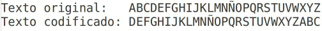
\includegraphics{top1}
  \label{fig:top1}
\end{figure}

{Para codificar un mensaje bastaba con buscar cada letra del mensaje original en la tabla anterior y  escribir la letra correspondiente del alfabeto cifrado. A la hora de decodificar el texto, se utilizaba la misma tabla pero buscando cada letra del texto codificado en el alfabeto original. Sencillo, pero para la época en que se utilizaba lo suficientemente seguro como para que el estado le confiase para mantener a salvo sus secretos.}
\\

{Hoy día, un cifrado como este sería rápidamente descubierto. En realidad, el cifrado de César puede ser atacado por el método de la “fuerza bruta”, simplemente tomando un trozo del texto y probando, uno a uno, todos los desplazamientos posibles que permita el alfabeto utilizado (unos 25 o 30, en general). Cuando se obtiene un texto que tiene sentido, se aplica ese desplazamiento al resto del documento y asunto resuelto.}
\\

\begin{center}
{VI.  REQUERIMIENTOS FUNCIONALES}
\end{center}

{Para nuestro código de encriptación y desencriptación de archivos se tendrá presente los siguientes requerimientos que permita la ejecución correcta de este código.} 

{Se utilizaran solamente archivo de texto (.txt) que contendrá solamente letras y contraseñas de cifrado de tipo string.}
\\

\textit{A. Clase cifrado:}

{• Se utiliza carácter tipo char para linea.}

{• Tipo string para el contenido del archivo (contenido), la clave de cifrado (clavecifrado) y la clave de descifrado
(clavedesen).}

{• Contendrá cadena de caracteres del archivo y el tamaño de este.}

{• Funciones que operaran con la clase principal como leer, encriptar, desencriptar, guardarencrip, guardadesncrip.}
\\

\textit{B. Leerarchivo():}

{• Será una función publica de la clase cifrado en la que tendrá la tarea de poder abrir el archivo especificado en la misma función.}

{• Leer los datos contenidos, analizar el tamaño del archivo para así cerrarlo.}
\\

\textit{C. Encriptar():}

{• Será una función publica de la clase cifrado, en donde se tendrá que ingresar una clave para así cifrar la información del archivo.}

{• Efectuara la trasformación del contenido del archivo.}
\\

\textit{D. Guardarencrip():}

{• Será una función publica de la clase cifrado, en donde se utilizaran dos archivos .txt para poder generar el guardado de los datos.}

{• Se podrá abrir los archivos para que este se escriban los datos que fueron con anterioridad encriptados.}
\\

\textit{E. Guardardesencrip():}

{• Será una función publica de la clase cifrado, donde se utilizaran dos archivos .txt.}

{• Leerá un archivo para que este pueda pasar la encriptación a otro archivo.}
\\

\textit{F. Desencriptar():}

{• Será una función publica de la clase cifrado, en donde Se implementara la clave de cifrado pedida anteriormente.}

{• Dicha clave se utilizará para dar acceso para el cifrado mientras esta sea errónea no se realizara nada.}
\\

\textit{G. Menu}

{• Será una función publica de la clase cifrado, que estará compuesto por selección del archivo, cifrar, descifrar y cerrar el programa.}

{• Ser crea un switch para que se vean las opciones que puede tener el usuario a la hora de ejecutar el programa.}

{• Necesitamos requerir de las funciones anteriores para que se realice lo que el código debe de hacer.}
\\

{Obteniendo así un código de cifrado, donde fijando un archivo podremos encriptar su información con una contraseña y desencriptarlo con esta misma.}
\\

\begin{center}
{VII. CONCLUSIONES}
\end{center}

{En conclusión, la criptografía es uno de los métodos para poder proteger la información, donde vuelve completamente ilegibles los datos de un archivo y de esa manera volverlo prácticamente inservible para un usuario no autorizado a leerlo, ya que si no cuenta con una contraseña de acceso no podrá verlo y mucho menos manipularlo. Hace parte de la seguridad informática donde hay diferentes métodos para proteger esta información como cifrado simétrico y asimétrico. La criptografía además es muy utilizada en el ámbito laboral, donde empresas la usan para proteger sus datos o archivos críticos y/o confidenciales.}
\\

{En este proyecto investigativo luego de analizar este método de seguridad de datos, se realizó un pequeño ejemplo donde podemos ver implementado esta técnica de seguridad de datos por medio del Cifrado Cesar, un tipo de cifrado utilizado en el pasado para la protección de datos importantes de personas no autorizadas, donde solo pocas personas conocían el método utilizado}
\\

{Y así comprobar la eficiencia de la criptografía para ocultar y proteger nuestros datos de personas no autorizadas para acceder a nuestra información privada.}

\begin{center}
{REFERENCIAS}
\end{center}

{[1] Marrero, Y. (2003). La Criptografía como elemento de la seguridad informática. ACIMED, 11(6). [Online]. Available: }
{http://scielo.sld.cu/scielo.php\?script\=sci_arttext\&pid\=S1024-94352003000600012\&lng\=es\&tlng\=es}
\\

{[2] ESET. (2014). Cifrado de la información. Guía Corporativa. [Online]. Available: }
{https://www.welivesecurity.com/wp\-content/uploads/2014/02/guia\_cifrado\_corporativo\_2014.pdf}
{\&ved\=2ahUKEwjAnMbYkqniAhVBwlkKHUXLC5YQFjAA}
{egQIAxAB\&usg\=AOvVaw0DVkxVuPpsRiik38eSMx79}
\\

{[3] Martínez. L.(2017). Algoritmo para la encriptacion y desencriptacion entre archivos digitales de audio e imagen. Universidad San Buenaventura Bogotá, D.C. [Online]. Available: }
{http://biblioteca.usbbog.edu.co:8080/Biblioteca/BDigital/}
{163087.pdf}
\\

{[4] IBM. Programa de Protección de Datos Críticos. [Online]. Available:}
{https://www.ibm.com/co-es/security/services/critical-data-protection-program}
\\

{[5] Myers, Lysa (2016). Todo sobre cifrado: qué es y cuándo deberías usarlo. ESET. [Online]. Available:}
{https://www.welivesecurity.com/la\-es/2016/02/09/todo\-sobre\-cifrado\-cuando\-usarlo/}
\\

{[6] Vázquez, C. (2015). Tipos de cifrado. [Online]. Available:}
{https://www.academia.edu/22411653/Tipos\_de\_Cifrado}
\\

{[7] Amador, S. Seguridad de la Información: Criptografia, Cifrado Cesar. [Online]. Available:}
{http://seguridad.unicauca.edu.co/criptografia/cifrado\_julio}
{\_cesar.pdf}

\end{document}
